\documentclass[aspectratio=169,xcolor=dvipsnames]{beamer}
\usetheme{SimpleDarkBlue}
\usepackage[T5]{fontenc}
\usepackage[utf8]{inputenc}
\usepackage{amsmath}
\usepackage{amssymb}
\usepackage{hyperref}
\usepackage{graphicx}
\graphicspath{{images/}}
\usepackage{booktabs}
\usepackage{array}

\title{Gradient Inversion Attacks in Federated Learning}
\subtitle{Deep Leakage from Gradients: Reconstructing Client Data from Shared Updates}
\author{}
\date{\today}

\begin{document}

\begin{frame}
\titlepage
\end{frame}

%------------------------------------------------
\begin{frame}{Outline}
\tableofcontents
\end{frame}

%------------------------------------------------

\section{Motivation \& Threat Model}

\begin{frame}{Outline}
\tableofcontents[currentsection]
\end{frame}

%------------------------------------------------

\begin{frame}{Federated Learning's Privacy Promise}
$K$ clients train a shared model without centralizing their data: each round, client
$k$ trains locally on private data $\mathcal{D}_k$ and returns only an update.
\[
w_{t+1} = w_t + \sum_{k \in S_t} \frac{n_k}{\sum_{j \in S_t} n_j} \, \Delta w_k^{(t)}
\]
\begin{itemize}
\item Only $\Delta w_k^{(t)}$ (or gradient $g_k^{(t)}$) is sent -- \textbf{raw data is
assumed to never leave the client}
\item Server just aggregates updates (FedAvg); this is the privacy claim we test
\end{itemize}
\end{frame}

%------------------------------------------------

\begin{frame}{The Gradient Inversion Problem}
An \textbf{honest-but-curious} attacker (the server itself, or an eavesdropper) follows
the protocol exactly, but tries to invert what it legitimately observes:
\[
g = \nabla_w \, \ell\big(w_t;\, \{x_i, y_i\}_{i=1}^{B}\big)
\;\;\longrightarrow\;\; \{(\hat{x}_i, \hat{y}_i)\}_{i=1}^{B}
\]
\begin{itemize}
\item \textbf{Knows:} architecture, loss $\ell$, weights $w_t$, leaked gradient $g$ \quad
\textbf{Does not know:} the private batch
\item Two answers to this problem: \emph{optimize} a dummy batch to match $g$, or
\emph{solve} for it directly in closed form
\end{itemize}
\end{frame}

%------------------------------------------------

\section{Attack Methods}

\begin{frame}{Outline}
\tableofcontents[currentsection]
\end{frame}

%------------------------------------------------

\begin{frame}{DLG: Deep Leakage from Gradients}
The first attack to show a leaked gradient alone is enough: search for a dummy batch
whose gradient matches the real one.
\[
\min_{\hat{x}, \hat{y}} \; \big\lVert g' - g \big\rVert_2^2,
\qquad g' = \nabla_w \, \ell(w_t; \hat{x}, \hat{y})
\]
\begin{itemize}
\item Dummy $(\hat{x}, \hat{y})$ start as random noise, jointly optimized by gradient
descent -- requires differentiating through $g'$ itself (``double backprop'')
\item Slow and occasionally unstable, since image and label are searched together
\end{itemize}
\end{frame}

%------------------------------------------------

\begin{frame}{iDLG: Closed-Form Label Recovery}
Same gradient-matching idea as DLG, but the label $\hat y$ no longer needs to be
searched for:
\[
\hat{y} = \arg\min_{c} \; \left(\frac{\partial \ell}{\partial z_c}\right)
\]
\begin{itemize}
\item For cross-entropy loss, the sign pattern of the last layer's gradient reveals the
true label in one step
\item Only the image $\hat{x}$ is then optimized against DLG's same objective -- faster,
more reliable convergence
\end{itemize}
\end{frame}

%------------------------------------------------

\begin{frame}{Inverting Gradients}
DLG's $L_2$ matching breaks down on deep nets, where gradient magnitude is dominated by
whichever layer is largest. Inverting Gradients matches \emph{direction} instead:
\[
\min_{\hat{x}} \; \left(1 - \frac{\langle g', g \rangle}{\lVert g' \rVert \, \lVert g \rVert}\right)
+ \alpha \, \mathrm{TV}(\hat{x})
\]
\begin{itemize}
\item Cosine cost + total-variation prior + sign-based Adam updates
\item This is what lets the attack scale to ImageNet-sized ResNet-18
\end{itemize}
\end{frame}

%------------------------------------------------

\begin{frame}{R-GAP: Recursive Gradient Attack on Privacy}
Instead of searching for a match at all, R-GAP solves for the input directly, one
layer at a time, from output back to input:
\[
z_l = W_l \, a_{l-1}, \quad a_l = \sigma(z_l), \qquad
\frac{\partial \ell}{\partial W_l} = \frac{\partial \ell}{\partial z_l} \, a_{l-1}^{\top}
\]
\begin{itemize}
\item Each layer's equation is solved exactly by linear algebra -- \emph{no}
optimization loop
\item Recovers $a_0 = x$ exactly, subject to each layer's rank/invertibility condition
\end{itemize}
\end{frame}

%------------------------------------------------

\section{DP-SGD Defense}

\begin{frame}{Outline}
\tableofcontents[currentsection]
\end{frame}

%------------------------------------------------

\begin{frame}{DP-SGD as a Post-Hoc Defense}
Reuses DP-SGD's clip-and-noise mechanics against exactly this leakage -- applied once
to the already-aggregated gradient, not the per-example, training-integrated,
formally-private mechanism of DP-SGD itself.
\[
\tilde{g} = \mathrm{clip}(g, C) + \mathcal{N}\!\big(0,\, (\sigma C)^2 I\big),
\qquad
\mathrm{clip}(g, C) = g \cdot \min\!\left(1, \frac{C}{\lVert g \rVert_2}\right)
\]
\begin{itemize}
\item Clip to global $L_2$ norm $C$, then add Gaussian noise of multiplier $\sigma$
\item Same $(C,\sigma)$ grid swept against every attack, to compare how much noise each
one tolerates
\end{itemize}
\end{frame}

%------------------------------------------------

\section{Experimental Evaluation}

\begin{frame}{Outline}
\tableofcontents[currentsection]
\end{frame}

%------------------------------------------------

\begin{frame}{Evaluation: Four Research Questions}
Each RQ primarily varies one factor relative to a shared anchor (LeNet, CIFAR-10, batch
1, no defense):
\begin{itemize}
\item \textbf{RQ1.} Same architecture, dataset, and batch size -- how do an
optimization-based attack (DLG/iDLG) and a closed-form attack (R-GAP) compare in
reconstruction quality and runtime?
\medskip
\item \textbf{RQ2.} Inverting Gradients is designed to scale -- does it still succeed
when the victim architecture is deeper and closer to practice (ResNet-18)?
\medskip
\item \textbf{RQ3.} How does each attack's reconstruction quality change when the
leaked gradient is averaged over a batch of two private images instead of one?
\medskip
\item \textbf{RQ4.} Can DP-SGD's clipping and noise suppress each attack, and does the
noise level needed to do so differ between attack families?
\end{itemize}
\end{frame}

%------------------------------------------------

\begin{frame}{Evaluation: Victim Configurations}
Every configuration evaluated across the four RQs:
\medskip
\resizebox{\linewidth}{!}{%
\begin{tabular}{@{}lllcc@{}}
\toprule
Method & Architecture & Dataset & Batch sizes & DP-SGD swept \\
\midrule
DLG / iDLG & LeNet (bias, sigmoid) & CIFAR-10 & 1, 2 & Yes \\
Inverting Gradients & ResNet-18 (untrained) & ImageNet (sample images) & 1, 2 & Yes \\
Inverting Gradients & LeNet (shared with DLG/iDLG) & CIFAR-10 & 1 & Yes \\
R-GAP & LeNetRGAP (bias-free, LeakyReLU) & CIFAR-10 & 1, 2 & Yes (batch 1 only) \\
R-GAP & FCN3 (bias-free, fully-connected) & CIFAR-10 (resized) & 2 & No \\
\bottomrule
\end{tabular}%
}
\bigskip
\begin{itemize}
\item The LeNet row shared by DLG/iDLG and Inverting Gradients uses identical
architecture, initial weights, and image -- giving RQ1 and RQ4 a matched-architecture
comparison point across the two attack families
\end{itemize}
\end{frame}

%------------------------------------------------

\begin{frame}{RQ1: Baseline Comparison, Shared LeNet}
All four methods, same LeNet, same image, batch size 1, no defense:
\begin{columns}[T]
\column{0.42\linewidth}
\small
\begin{tabular}{@{}lcc@{}}
\toprule
Method & MSE & PSNR \\
\midrule
DLG & 0.00140 & 28.55 dB \\
iDLG & 0.00160 & 27.95 dB \\
Inv.\ Gradients & 0.0022 & 26.48 dB \\
R-GAP & $<10^{-7}$ & $\infty$ (exact) \\
\bottomrule
\end{tabular}
\column{0.56\linewidth}
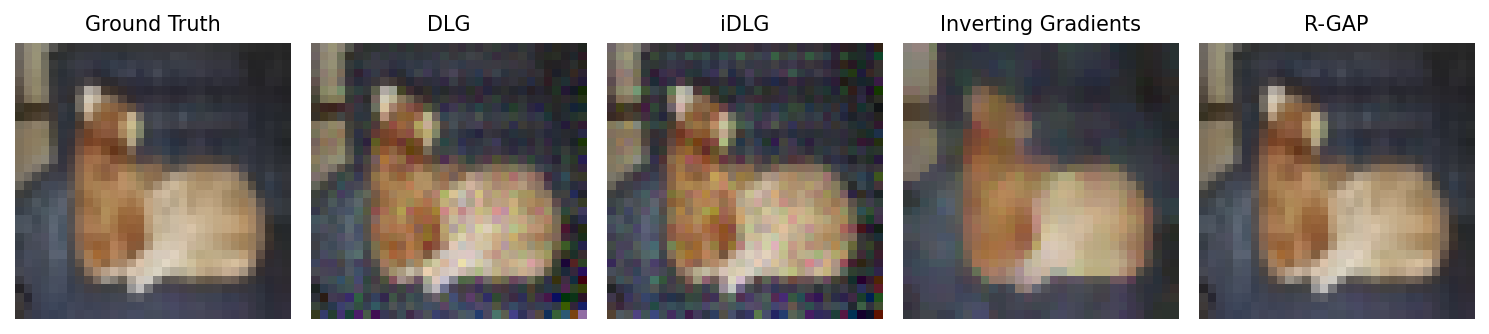
\includegraphics[width=\linewidth]{rq1_all_methods.png}
\end{columns}
\end{frame}

%------------------------------------------------

\begin{frame}{RQ1: Convergence of DLG vs.\ iDLG}
Both start from the same random noise; this is how they reach the result above.
\centering
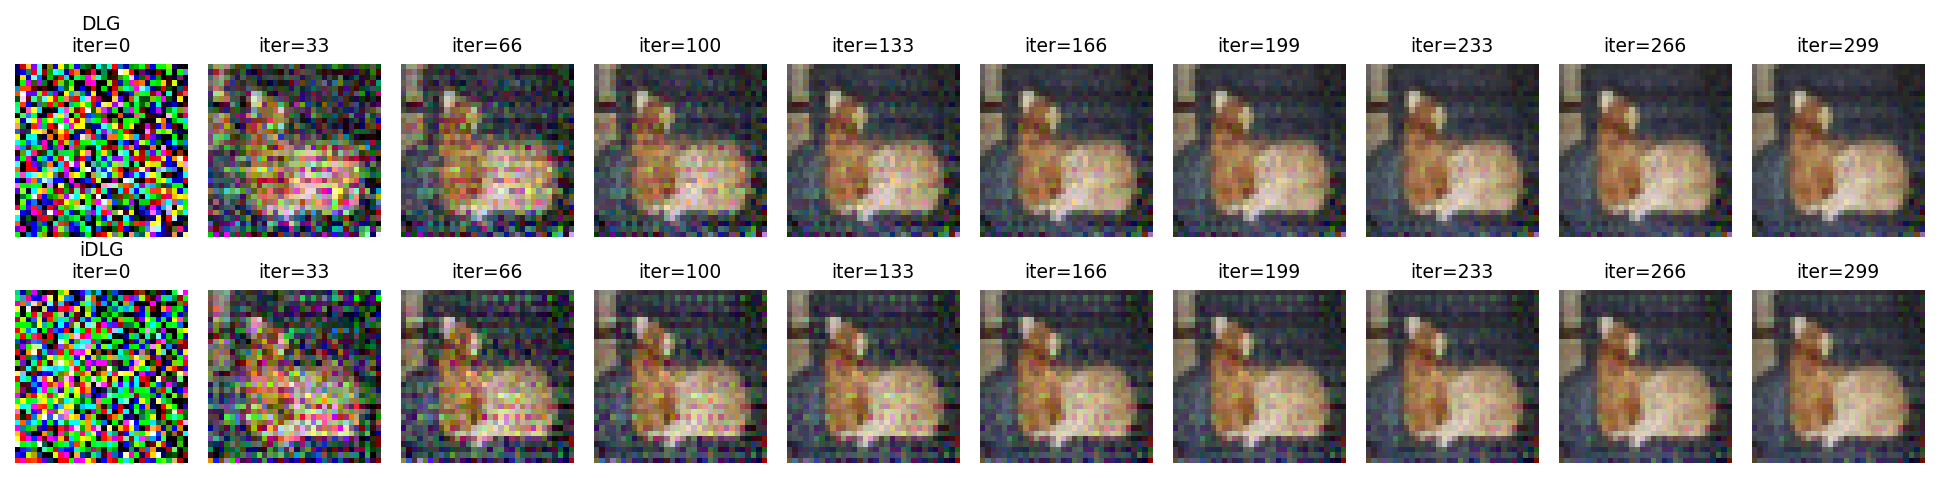
\includegraphics[width=.92\linewidth,height=.6\textheight,keepaspectratio]{rq1_milestones.png}
\begin{itemize}
\small
\item 10 milestones over the same 300-iteration L-BFGS run
\item iDLG's single-variable search settles into shape earlier than DLG's joint search
\end{itemize}
\end{frame}

%------------------------------------------------

\begin{frame}{RQ1: R-GAP Needs Float64}
R-GAP's exactness above is conditional on precision -- repeating it in float32 fails:
\centering
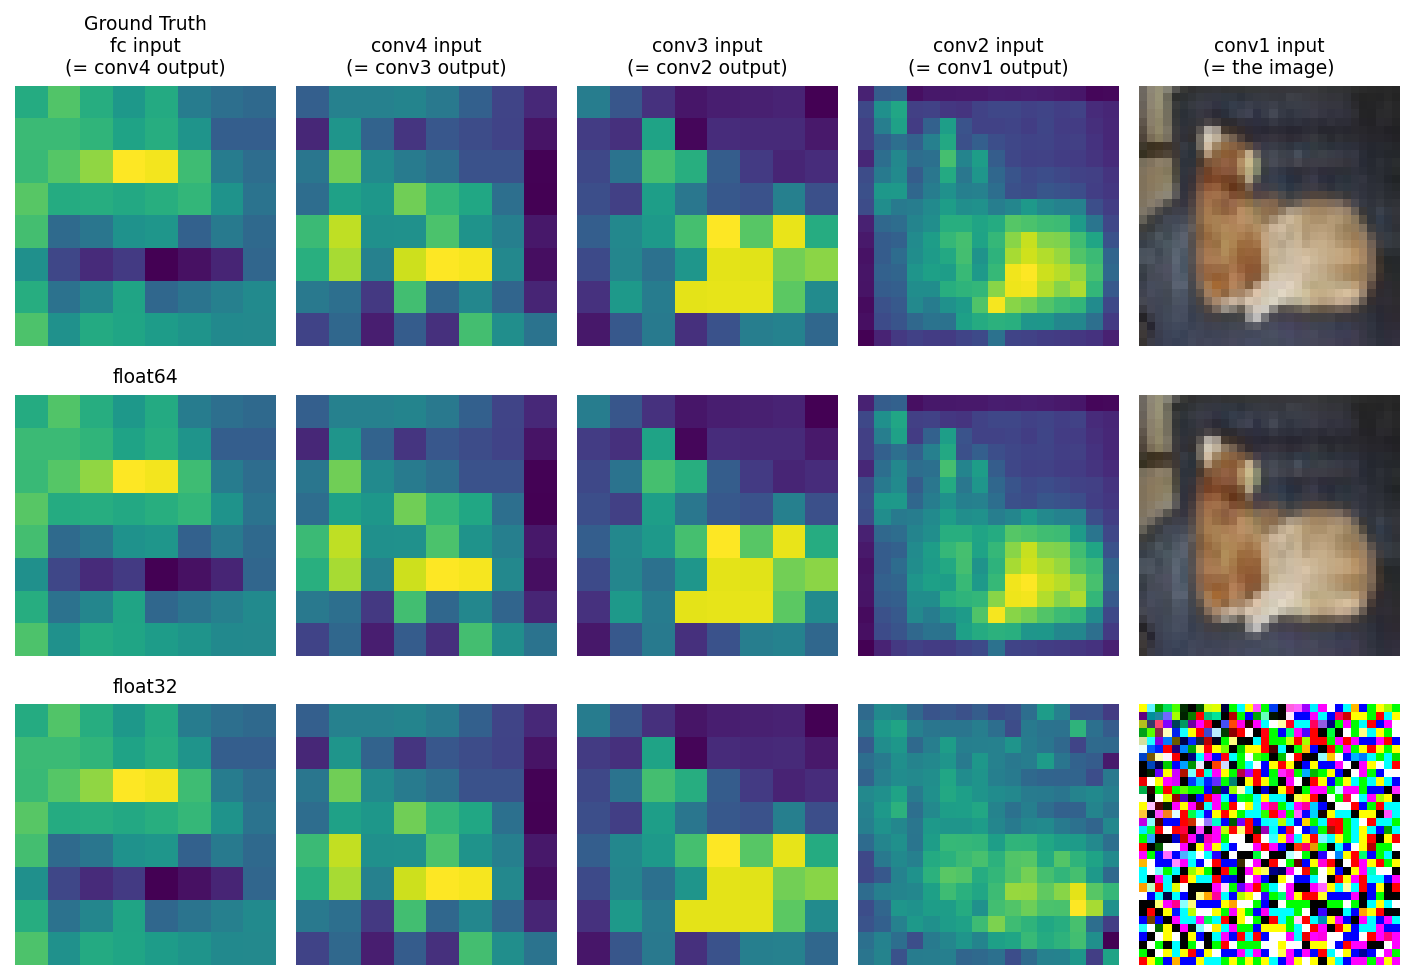
\includegraphics[width=.9\linewidth,height=.55\textheight,keepaspectratio]{rq1_rgap_float.png}
\begin{itemize}
\small
\item float64: exact (MSE $<10^{-7}$) \quad vs.\quad float32: MSE $=91.25$, PSNR $=-19.6$ dB
\item Failure localized to the final linear solve, where the smallest singular value
amplifies rounding error
\end{itemize}
\end{frame}

%------------------------------------------------

\begin{frame}{RQ2: Scaling to ResNet-18}
Does Inverting Gradients' design actually deliver at a realistic scale?
\centering
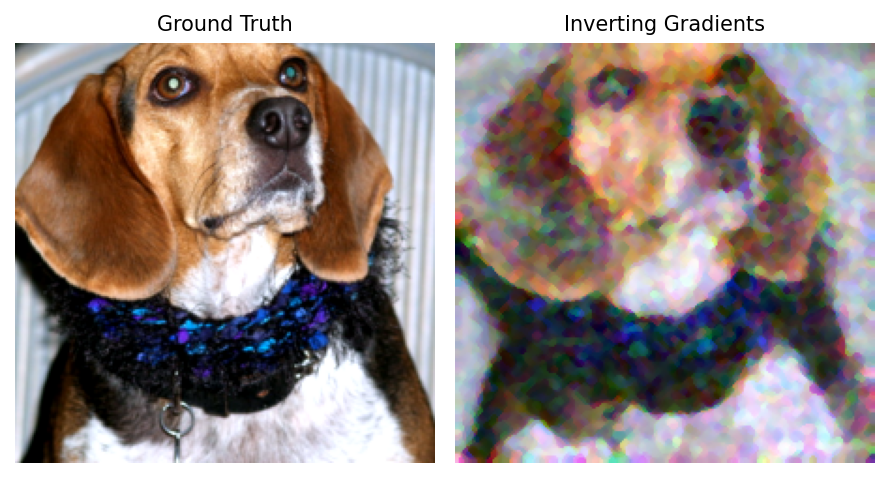
\includegraphics[width=.5\linewidth,height=.55\textheight,keepaspectratio]{rq2_ig_resnet18.png}
\begin{itemize}
\small
\item Untrained ResNet-18, 11.7M params, $224{\times}224$ image -- an order of magnitude
larger than RQ1's LeNet
\item MSE $=0.0185$, PSNR $=17.33$ dB -- visibly identifiable, but well below RQ1's
26.48 dB on the smaller network
\end{itemize}
\end{frame}

%------------------------------------------------

\begin{frame}{RQ3: Batch Size 1 vs.\ 2 -- Optimization-Based Attacks}
Each attack is compared against its own batch-size-1 result, when the leaked gradient
instead averages two private images:
\medskip
\centering
\begin{tabular}{@{}lcc@{}}
\toprule
Method (architecture) & Batch 1 (PSNR) & Batch 2 (mean PSNR) \\
\midrule
DLG (LeNet) & 28.55 dB & 16.29 dB \\
iDLG (LeNet) & 27.95 dB & 16.65 dB \\
Inverting Gradients (ResNet-18) & 17.33 dB & 16.35 dB \\
\bottomrule
\end{tabular}
\bigskip
\begin{itemize}
\item Both LeNet attacks lose roughly 11--12 dB going from batch 1 to batch 2
\item Inverting Gradients on ResNet-18 loses under 1 dB -- its batch-1 result was
already far from perfect (RQ2), leaving less margin left to lose
\end{itemize}
\end{frame}

%------------------------------------------------

\begin{frame}{RQ3: Inverting Gradients, ResNet-18, Batch Size 2}
\centering
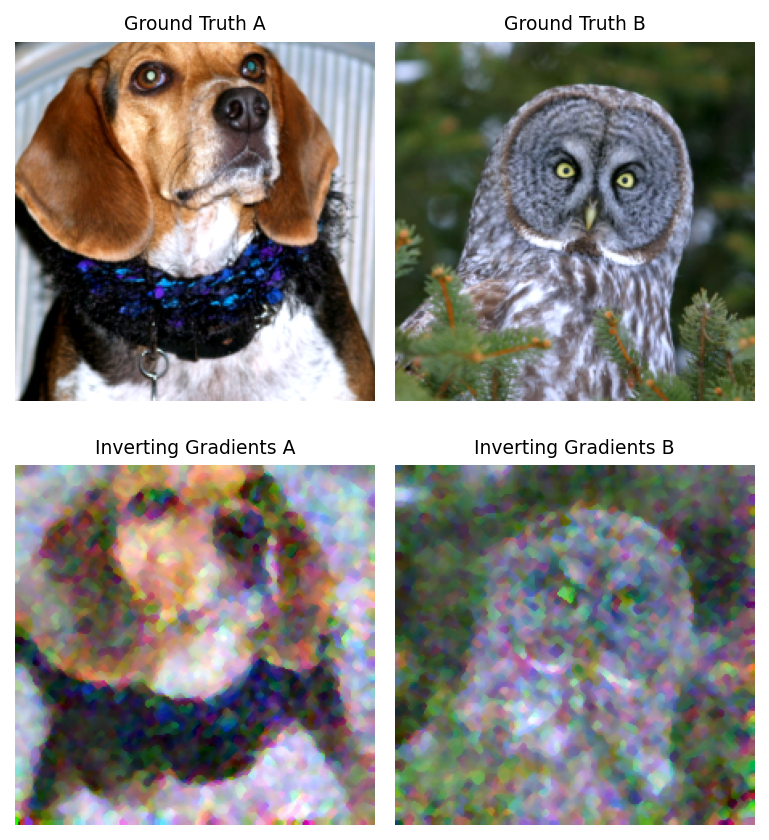
\includegraphics[width=.75\linewidth,height=.68\textheight,keepaspectratio]{rq3_ig_resnet18_batch2.png}
\begin{itemize}
\small
\item Both batch-2 reconstructions remain individually identifiable, despite the small
PSNR drop from batch 1
\end{itemize}
\end{frame}

%------------------------------------------------

\begin{frame}{RQ3: R-GAP at Batch Size 2 -- the Linear-Combination Property}
With $B=2$ the leaked gradient averages both images -- does R-GAP's exact solve
degrade the same way on every architecture?
\medskip
\centering
\begin{tabular}{@{}lccc@{}}
\toprule
& \multicolumn{3}{c}{Cosine similarity to ground truth} \\
Architecture & vs.\ image A & vs.\ image B & vs.\ average $(A{+}B)/2$ \\
\midrule
LeNetRGAP (CNN) & 0.062 & 0.055 & 0.061 \\
FCN3 (fully-connected, LeakyReLU) & 0.959 & 0.967 & 1.000 \\
\bottomrule
\end{tabular}
\bigskip
\begin{itemize}
\item On FCN3 (no conv layers), R-GAP's recursive solution closely matches the
\emph{direction} of the average of the two inputs -- R-GAP inverts its LeakyReLU
exactly, so nonlinearity isn't what matters here
\item A convolutional architecture (LeNetRGAP) adds extra forward-pass constraints that
this blended, two-image signal does not satisfy -- the reconstruction matches neither
image nor their average
\end{itemize}
\end{frame}

%------------------------------------------------

\begin{frame}{RQ3: R-GAP Batch-2 Reconstructions}
\centering
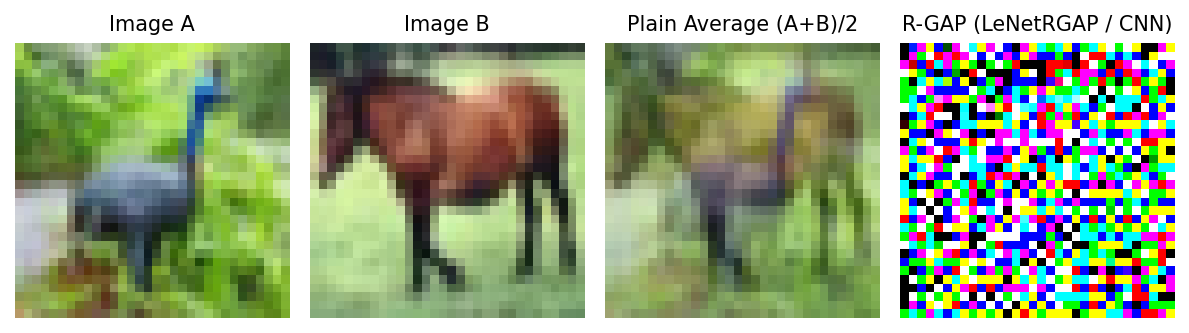
\includegraphics[width=.8\linewidth,height=.36\textheight,keepaspectratio]{rq3_rgap_cnn_batch2.png}\\[0.4em]
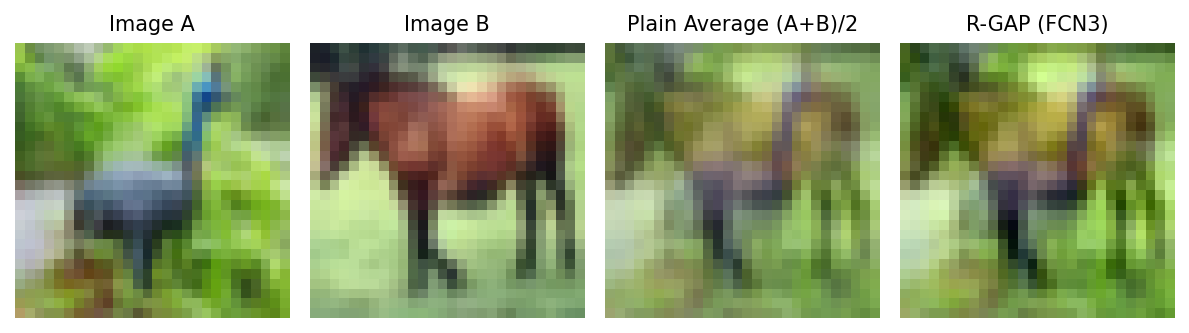
\includegraphics[width=.8\linewidth,height=.36\textheight,keepaspectratio]{rq3_rgap_fcn3_batch2.png}
\begin{itemize}
\small
\item LeNetRGAP/CNN (top): visibly uncorrelated noise
\item FCN3 (bottom): closely matches the direction of the pixel average
\end{itemize}
\end{frame}

%------------------------------------------------

\begin{frame}{RQ4: DP-SGD vs.\ DLG Family (LeNet)}
Same $(C,\sigma)$ grid, same LeNet -- does clipping/noise hit the $L_2$ and cosine cost
functions equally hard?
\medskip
\centering
\begin{tabular}{@{}lcccc@{}}
\toprule
& \multicolumn{4}{c}{PSNR (dB) at $C=1.0\lVert g\rVert$ (no clipping)} \\
Method (architecture) & $\sigma=0$ & $10^{-4}$ & $10^{-3}$ & $10^{-2}$ \\
\midrule
iDLG (LeNet) & 16.14 & 14.05 & $-8.11$ & $-18.83$ \\
Inverting Gradients (LeNet) & 27.94 & 27.32 & 17.34 & 10.75 \\
Inverting Gradients (ResNet-18) & 12.72 & 12.17 & 9.71 & 9.43 \\
\bottomrule
\end{tabular}
\bigskip
\begin{itemize}
\item Clipping alone already separates the two costs: iDLG's $L_2$ cost is sensitive to
the gradient's magnitude and collapses under aggressive clipping even at $\sigma=0$;
Inverting Gradients' cosine cost is scale-invariant and barely changes
\item Increasing $\sigma$ then degrades both, but iDLG collapses sharply between
$10^{-4}$ and $10^{-3}$, while Inverting Gradients stays above 17 dB at that point
\end{itemize}
\end{frame}

%------------------------------------------------

\begin{frame}{RQ4: Reconstructions Under DP-SGD (LeNet)}
\centering
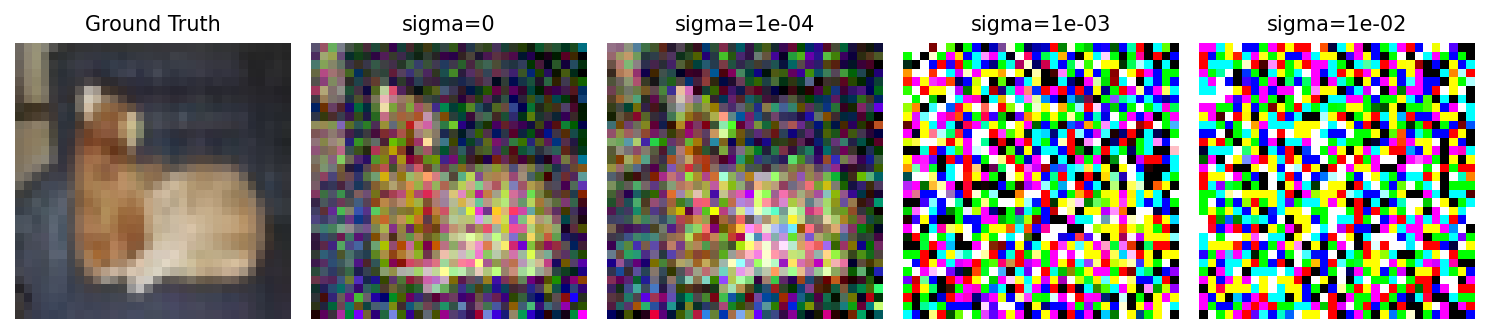
\includegraphics[width=.85\linewidth,height=.4\textheight,keepaspectratio]{rq4_idlg_grid.png}\\[0.4em]
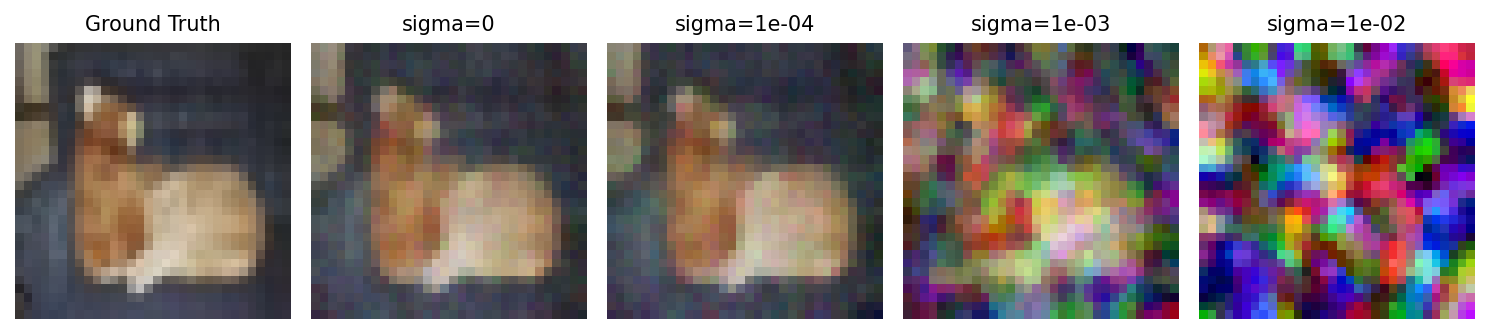
\includegraphics[width=.85\linewidth,height=.4\textheight,keepaspectratio]{rq4_ig_lenet_grid.png}
\begin{itemize}
\small
\item iDLG (top) turns to pure noise well before Inverting Gradients (bottom) does, at
the same noise levels
\end{itemize}
\end{frame}

%------------------------------------------------

\begin{frame}{RQ4: DP-SGD vs.\ R-GAP}
R-GAP needs a far finer noise grid than the attacks above -- the same grid would
overshoot its breaking point entirely and show nothing but collapse:
\medskip
\centering
\begin{tabular}{@{}lcccccc@{}}
\toprule
& \multicolumn{6}{c}{PSNR (dB) at $C=1.0\lVert g\rVert$ (no clipping)} \\
$\sigma$ & 0 & $10^{-9}$ & $10^{-8}$ & $10^{-7}$ & $10^{-6}$ & $10^{-5}$ \\
\midrule
R-GAP (LeNetRGAP) & $\infty$ & 73.2 & 51.6 & 31.0 & $-19.5$ & $-18.5$ \\
\bottomrule
\end{tabular}
\bigskip
\begin{itemize}
\item Exact at $\sigma=0$, as in RQ1; still 31.0 dB at $\sigma=10^{-7}$
\item Collapses to $-19.5$ dB at $\sigma=10^{-6}$ -- just one order of magnitude more
noise, three to four orders of magnitude below where iDLG breaks
\end{itemize}
\end{frame}

%------------------------------------------------

\begin{frame}{RQ4: R-GAP Reconstructions Under DP-SGD}
\centering
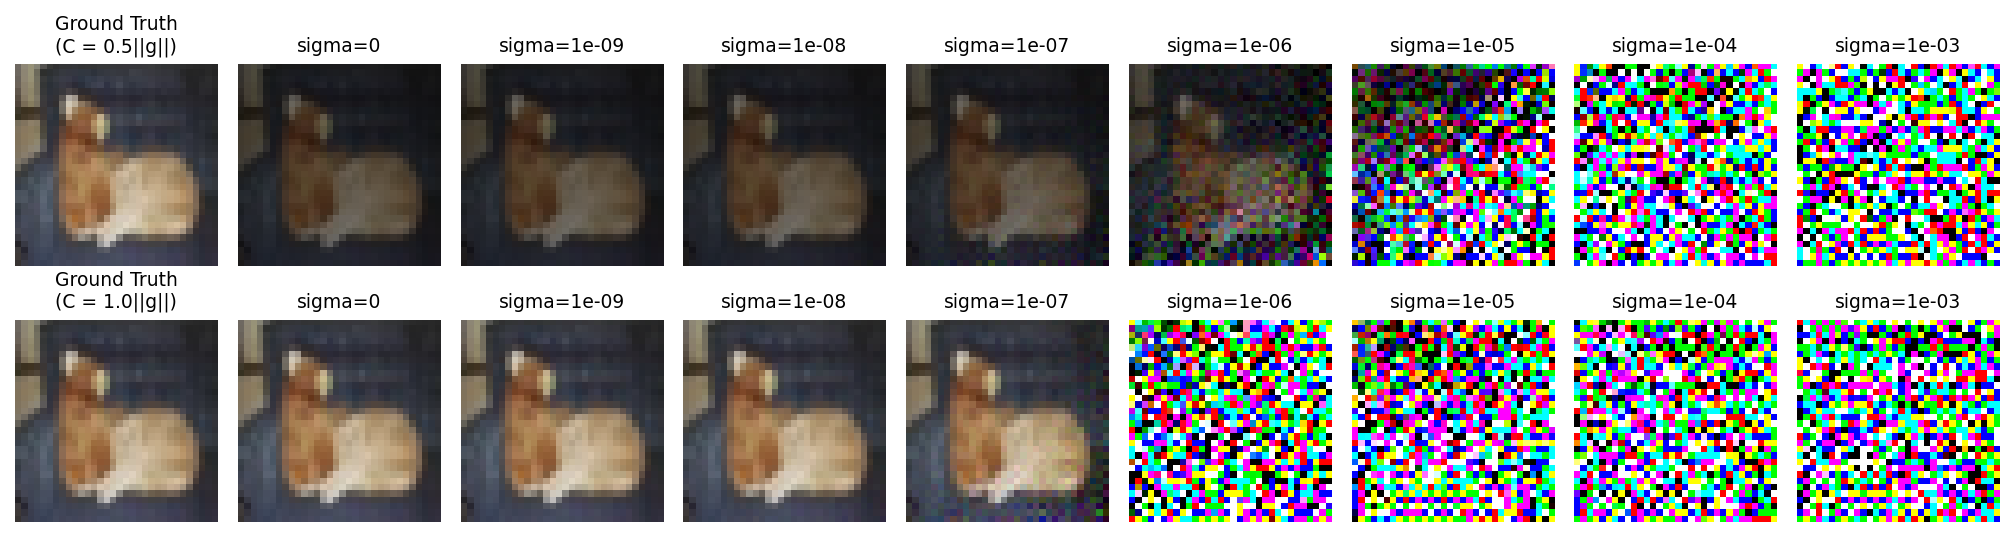
\includegraphics[width=.95\linewidth,height=.68\textheight,keepaspectratio]{rq4_rgap_grid.png}
\begin{itemize}
\small
\item The break between $\sigma=10^{-7}$ and $10^{-6}$ is visible by eye, at a noise
level too small to touch DLG, iDLG, or Inverting Gradients at all
\end{itemize}
\end{frame}

%------------------------------------------------

\section{Conclusion}

\begin{frame}{Outline}
\tableofcontents[currentsection]
\end{frame}

%------------------------------------------------

\begin{frame}{Key Takeaways}
\begin{itemize}
\item Gradients alone are enough to reconstruct private images/labels
\item Closed-form (R-GAP) is exact and fastest, but fragile: precision and batch size
\item Optimization-based attacks scale further but converge less precisely
\item DP-SGD noise that defeats R-GAP leaves DLG/iDLG visibly unaffected
\item No single defense budget suppresses every attack family equally
\end{itemize}
\end{frame}

%------------------------------------------------

\begin{frame}
\begin{center}
{\Large \textbf{Thank You}}\\[1em]
{\large Questions?}
\end{center}
\end{frame}

%------------------------------------------------

\end{document}
